
\begin{picture} (180.000000,180.000000)(0,0)
\put(0.0, 0.0){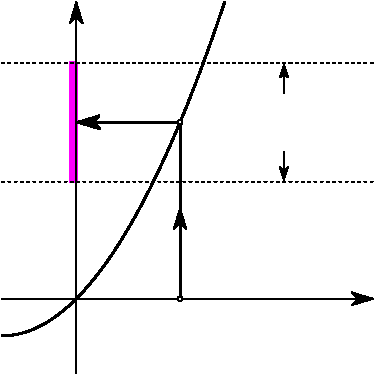
\includegraphics{03epsAndNoDelta.pdf}}
    \put( -2.00,  92.85){\sffamily\itshape \makebox[0pt][r]{$L-\varepsilon$}}
    \put( -2.00, 149.81){\sffamily\itshape \makebox[0pt][r]{$L+\varepsilon$}}
    \put( 31.60, 121.33){\sffamily\itshape \makebox[0pt][r]{$L$}}
    \put(108.24, 168.50){\sffamily\itshape $y=f(x)$}
    \put( 84.44,  24.60){\sffamily\itshape $a$}
    \put( 91.44, 121.33){\sffamily\itshape \
How close must $x$ be to $a$ for $f(x)$ to end up in this range?
}
\end{picture}
